% \begin{center}
\documentclass[12pt]{article}
\usepackage[letterpaper, left=1.25in, right=1.0in, top=1.25in, bottom=1.1in]{geometry} %% set margins are the template
\usepackage{fullpage,setspace}
\usepackage{hyperref, url}
\usepackage[hang,flushmargin]{footmisc} %control footnote indent
\usepackage{amssymb,amsmath}%for matrix
\usepackage{graphicx,float,morefloats,rotfloat,lscape}%for figure
\usepackage{subfig}
\usepackage{multirow}
\usepackage{longtable,rotating}
\usepackage{caption}
\usepackage{color}
\usepackage[round]{natbib} % for citation style, round brackets
\usepackage{listings}
\usepackage{courier}
\usepackage{color}
\usepackage{mwe}
\captionsetup[subtable]{font=normal}
\usepackage[export]{adjustbox}
\usepackage{bm}
\usepackage{appendix}

\usepackage[absolute]{textpos}
\usepackage{fancyhdr}

\usepackage{titling}
\pretitle{\begin{center}\huge}
\posttitle{\par\end{center}}
\preauthor{\normalfont\normalsize\begin{center}\begin{tabular}[t]{c}}
\postauthor{\end{tabular}\end{center}}

\setlength{\parindent}{0em}
\setlength{\parskip}{0.5em}
\floatstyle{plaintop}
\restylefloat{table}
\captionsetup[subtable]{font=normal}
\graphicspath{{0.plots/}}
\doublespace

\fancypagestyle{lscape}{%
\fancyhf{} % clear all header and footer fields
\fancyfoot[LE]{%
\begin{textblock}{20}(1,5){\rotatebox{90}{\leftmark}}\end{textblock}
\begin{textblock}{1}(13,7.5){\rotatebox{90}{\thepage}}\end{textblock}
}
\fancyfoot[LO] {%
\begin{textblock}{1}(13,7.5){\rotatebox{90}{\thepage}}\end{textblock}
\begin{textblock}{20}(1,13.25){\rotatebox{90}{\rightmark}}\end{textblock}
}
\renewcommand{\headrulewidth}{0pt}
\renewcommand{\footrulewidth}{0pt}}


\begin{document}

\title{Bayesian Quantile Regression Joint Models of Longitudinal and Recurrent Event Data}


\author{}
\date{}

\maketitle


\begin{center}
{\bf Abstract}
\end{center}

Recurrent event outcome (e.g. multiple heart failures, cancer recurrences, hospital readmissions, etc.) is commonly encountered in longitudinal biomedical studies. In those studies, recurrent event outcome can be an important outcome of interest in monitoring disease progression or health condition of the study participants in addition to other continuous longitudinal outcome. For example, in the Atherosclerosis Risk In Communities Study (ARIC), recurrent event outcomes, including coronary heart disease, stroke, and heart failure, etc., were collected from extensive cohort surveillance to monitor the health condition of the study cohort; meanwhile, repeated systolic blood pressure (SBP) were also measured at regular clinical visits as a disease biomarker. Previous studies using ARIC data found positive correlation between SBP and recurrent CHD events in the study cohort. This data mechanism motivates us to consider the joint models (JM) of longitudinal and recurrent event data. JM models the bivariate outcomes jointly in accounting for the correlation between them, while studying potential disease risk factors for both outcomes simultaneously. In the traditional JM framework, a linear mixed model (LMM) is commonly used for the longitudinal outcome. LMM assumes normal random error; however, in many circumstances, the normality assumption cannot be satisfied and the it is not appropriate to use directly. Moreover, LMM only models the conditional mean of the longitudinal outcome, which may not be desirable in many clinical studies. In contrast to mean regression, quantile regression (QR) provides a more flexible, distribution-free way to study covariate effects at different quantiles of the longitudinal outcome. This becomes extremely important when higher (e.g. SBP) or lower (e.g. CD4 count) tail of the outcome is more relevant to clinical interest. In this paper, we propose to use the so-called linear quantile mixed model (LQMM) for the longitudinal outcome jointly with a proportional hazard model (PHM) for the recurrent event outcome under the JM framework. We develop a Gibbs sampling algorithm for model inference, which is based on the location-scale representation of the asymmetric Laplace distribution for LQMM. We assess the performance of our Bayesian algorithm through extensive simulation study and applied the proposed model to the longitudinal SBP and recurrent CHD event data from the ARIC Study.

{\bf Key words:} Bayesian; Joint models; Linear quantile mixed model; Recurrent event.


\section{Introduction}
Recurrent event, such as multiple cardiovascular diseases (CVD), cancer recurrences, and hospital readmissions, are commonly encountered in clinical studies. Meanwhile, during the follow-up, some longitudinal outcomes are usually measured repeatedly at regular clinical visits or when events occur. It is common that longitudinal biomarkers are informative for the occurrence of repeated events in many clinical settings. As a typical example, patients with higher blood pressure (BP) are more likely to experience coronary heart diseases (CHD) \citep{wattanakit2005risk, rodriguez2014systolic}. Ignoring the dependence between the longitudinal and recurrent event processes and the fit models for the two outcomes separately will lead to loss of information and result in biased or inefficient inference results. Traditional survival model with time-varying covariate may not be appropriate to use due to its limiting assumption of external time-dependent covariates that are not related to the event mechanism. In contrast, joint models (JM) of longitudinal and recurrent event data is more appropriate to use to study the association between the two processes and to model the two outcomes simultaneously.

Joint analysis of longitudinal and time-to-event outcome has been studied by many authors. However, majority of the literature focuses on JM of longitudinal and a single time-to-event (e.g. terminal event). For example, \cite{self1992modeling, tsiatis1995modeling, wulfsohn1997joint} developed the JM methods for survival analysis with a time dependent covariate measured with error. \cite{tsiatis2004joint} gives an excellent review of such JM method. With more recent development, \cite{rizopoulos2011dynamic,taylor2013real} introduced the novel idea of making subject-specific dynamic predictions of future event-free probability based on the JM of longitudinal continuous outcome and survival. In contrast, joint analysis of longitudinal and recurrent event outcomes has received less attention so far. To our knowledge, \cite{henderson2000joint} developed a JM for longitudinal data with either terminal or recurrent event but not for both. \cite{efendi2013joint} proposed a JM of longitudinal and recurrent event outcomes that accommodates overdispersion.

In traditional JM, the longitudinal continuous outcome is commonly modeled using a linear mixed model (LMM) \citep{laird1982random}; while possible violation to the normality assumption in the error term is not considered. Moreover, an LMM  models covariate effects on the conditional mean of the outcome; however, in many clinical settings it is more desirable that we can make inference at lower or higher quantiles of the outcome. For example, researchers used quantile regression (QR) models to study covariate effects on lower birth weight, which turned out to be significantly different compared with that on the mean birth weight \citep{koenker2001quantile}. In contrast to linear regression, QR is a more flexible tool that relaxes the distributional assumption, and provides a way to study covariate effects on various conditional quantiles of the outcome \citep{koenker2005quantile}. This feature find its great importance in biomedical studies, where individuals with extremer biomarker measurements are often at higher risk of disease or death. To our knowledge, \cite{farcomeni2015longitudinal} is the first one to incorporate a linear quantile mixed model (LQMM) into a JM of longitudinal and terminal event data, in which they developed a Monte Carlo Expectation Maximization (MCEM) algorithm for parameter estimation. However, there is little work has been do to use LQMM in the joint analysis of longitudinal and recurrent event data so far.

In this paper, we propose a new version of JM for analyzing longitudinal and recurrent event data jointly, in which we adopt the LQMM in modeling the longitudinal continuous outcome and use the the proportional hazard model (PHM) for recurrent event outcome. In this JM, the longitudinal outcome is treated as a time-dependent covariate in the time-to-event model and the dependence is measured by some association parameter. Differently from \cite{farcomeni2015longitudinal}, we develop a Gibbs sampling algorithm for model inference. Development of the fully Bayesian algorithm is based on the fact that minimizing the original QR loss function is equivalent to maximizing the likelihood function of the so-called asymmetric Laplace distribution (ALD) \citep{yu2001bayesian}. Moreover, the ALD can be further reparameterized using a location-scale mixture representation that leads to a combination of normal and exponential distributions \citep{kotz2001laplace, kozumi2011gibbs}. The proposed Bayesian estimating algorithm can be directly implemented in existing software. In application, we use the data derived from the Atherosclerosis Risk in Communities Study (ARIC) to demonstrate our proposed model. ARIC is a prospective epidemiologic study conducted to investigate the etiology of atherosclerosis and its clinical outcomes, and variation in cardiovascular risk factors, medical care, and disease by race, gender, location, and date. And we apply the proposed JM to study various covariates effect on different quantiles of the systolic blood pressure (SBP) as well as the association between SBP and the recurrence of coronary heart disease (CHD).

The rest of this paper is organized as follows. In Section \ref{sec:p2methods}, we give details of the proposed statistical model and the Bayesian algorithm used for model inference. In Section \ref{sec:p2simulation}, we present simulation study to validate the proposed methods. In Section \ref{sec:p2data}, we apply the proposed methods to the ARIC data. We conclude the paper with a discussion in Section \ref{sec:p2discussion}.





\section{Methods}\label{sec:p2methods}
% \renewcommand{\thesubsection}{\thesection.\arabic{subsection}}
%%%%%%%%%%%%%%%%%%%%%%%%%%%
\subsection{Bayesian Linear Quantile Mixed Model}\label{sec:p2BLQMM}
Let $Y_{i}(t_{ij})$ be the longitudinal outcome for subject $i$ measured at time $t_{ij}$ where $i=1, \cdots, N\mbox{ and } j=1,\cdots, n_i$. Consider the linear mixed effects model:
\begin{equation}\label{eqn:p2lmm}
Y_{i}(t) ={\boldsymbol X}_{i}^{\top}(t) \boldsymbol{\beta}+ {\boldsymbol Z}_{i}^{\top}(t)\boldsymbol{u}_i + \varepsilon_{i}(t),
\end{equation}

\noindent where $\boldsymbol{\beta}$ is a $p-$dimensional vector of fixed effects,  ${\boldsymbol X}_{i}(t)$ contains the corresponding fixed covariates, $\boldsymbol{u}_i$ is a $k-$dimensional vector of random effects for subject $i$, and ${\boldsymbol Z}_{i}(t)$ are the corresponding random covariates.

An LQMM assumes that the conditional quantile of the outcome is a linear function of the covariates, i.e.,
\begin{equation}\label{eqn:p2lqmm}
Q_{Y_{i}(t)|{\boldsymbol X}_{i}(t),{\boldsymbol Z}_{i}(t)}(\tau)={\boldsymbol X}_{i}^{\top}(t) \boldsymbol{\beta}+ {\boldsymbol Z}_{i}^{\top}(t)\boldsymbol{u}_i,
\end{equation}

\noindent where the $\tau$th quantile of a random variable $Y$ is defined as $Q_{Y}(\tau)=F_{Y}^{-1}(\tau)=\inf\left\{ y:F_{Y}(y)\geq\tau\right\}$, for $\tau\in [0, 1]$. Parameter estimations can then be obtained by minimizing the following loss function,

\begin{equation*}\label{eqn:p2loss_fun}
\hat{\boldsymbol{\beta}}_{\tau}=\underset{\boldsymbol{\beta}\in \mathbb{R}^{p}}{\mbox{arg min}}\sum_{i, t}\left[\rho_{\tau}\left(Y_{i}(t)-{\boldsymbol X}_{i}^{\top}(t)\boldsymbol{\beta} - {\boldsymbol Z}_{i}^{\top}(t)\boldsymbol{u}_i\right)\right],
\end{equation*}

\noindent where $\rho_{\tau}(\cdot)$ is defined as $\rho_{\tau}(Y)=Y(\tau-{I}{(Y<0)}).$

Above minimization problem can be rephrased as a maximum-likelihood problem by assuming the random error $\varepsilon_{i}(t)$ in (\ref{eqn:p2lmm}) follows ALD with location parameter equals 0, scale parameter $\sigma$ and skewness parameter $\tau$ \citep{koenker1999goodness,yu2001bayesian}:
\begin{equation*}
Y_{i}(t) ={\boldsymbol X}_{i}^{\top}(t) \boldsymbol{\beta}+ {\boldsymbol Z}_{i}^{\top}(t)\boldsymbol{u}_i + \varepsilon_{i}(t), \varepsilon_{i}(t)\sim ALD(0, \sigma, \tau).
\end{equation*}

This becomes clear when writing out the conditional likelihood function:
\begin{equation*}\label{eqn:p2ald_lqmm}
f(Y_{i}(t)|\boldsymbol{\beta}_{\tau},\boldsymbol{u}_i,\sigma)=\frac{\tau(1-\tau)}{\sigma}\exp\left[-\rho_{\tau}\left(\frac{Y_{i}(t)-{\boldsymbol X}_{i}^{\top}(t)\boldsymbol{\beta}_{\tau}-{\boldsymbol Z}_{i}^{\top}(t)\boldsymbol{u}_i}{\sigma}\right)\right].
\end{equation*}

In Bayesian quantile regression context a Gibbs sampling algorithm for model inference can be developed when we utilize a location-scale mixture representation of the ALD \citep{kotz2001laplace}. Under such parameterization the random error is represented as $\varepsilon_{i}(t)=\kappa_1e_{i}(t)+\kappa_2\sqrt{\sigma e_{i}(t)}v_{i}(t)$ with $v_{i}(t)\sim N(0,1), e_{i}(t)\sim\exp(1/\sigma)$ and
\[\kappa_1=\frac{1-2\tau}{\tau(1-\tau)}\hspace{2em} \kappa_2^2=\frac{2}{\tau(1-\tau)}.\]


This reparameterization leads to the following linear mixed model,
\begin{equation*}\label{eqn:p2reformald2}
Y_{i}(t)={\boldsymbol X}_{i}^{\top}(t)\boldsymbol{\beta}_{\tau}+{\boldsymbol Z}_{i}^{\top}(t)\boldsymbol{u}_i+\kappa_1e_{i}(t)+\kappa_2\sqrt{\sigma e_{i}(t)}v_{i}(t),
\end{equation*}
\noindent or equivalently,
{\small
\begin{equation}\label{eqn:p2lo_sc_lh}
f(Y_{i}(t)|\boldsymbol{\beta}_{\tau},\boldsymbol{u}_i,e_{i}(t),\sigma)=\frac{1}{\sqrt{2\pi\kappa_2^2\sigma e_{i}(t)}}\exp\left[-\frac{(Y_{i}(t)-{\boldsymbol X}_{i}^{\top}(t)\boldsymbol{\beta}_{\tau}-{\boldsymbol Z}_{i}^{\top}(t)\boldsymbol{u}_i-\kappa_1e_{i}(t))^2}{2\kappa_2^2\sigma e_{i}(t)}\right].
\end{equation}
}

As discussed in \cite{yu2001bayesian}, irrespective of the actual distribution of the data, Bayesian quantile regression using ALD distribution works quite well for different error distributions and the performance is quite robust and satisfactory.

%%%%%%%%%%%%%%%%%%%%%%%%%%%
\subsection{Joint Models Using Longitudinal Quantile Regression}
For subject $i$, let $T_{ik}^*$ be the underlying true $k$th recurrent event time and $C_i$ be the censoring time, which is assumed to be independent of both outcomes. Then $T_{ik} = $\mbox{ min}($C_i, T_{ik}^*)$, for $k=1, \cdots, m_i$, is the observed $k$th event time, where $m_i$ is the total number of recurrent events for subject $i$. Let $\delta_{ik}$ be the recurrent event indicator at time $T_{ik}$ which is defined as $\delta_{ik} = I(T_{ik}^* < C_i)$, and $I(\cdot)$ is the indicator function. A $k$th recurrent event is observed at time $T_{ik}$ if $\delta_{ik}=1$, i.e. $T_{ik}^* < C_i$; other wise, $\delta_{ik}=0$.

Let $Y_{i}(t)$ be the continuous longitudinal outcome for subject $i$ measured at time $t$. Note that we can only observe $Y_{i}(t)$ when $t\le C_i$, and the complete longitudinal trajectory up to follow-up time $t$ for subject $i$ can be written as $\mathcal{Y}_{i}(t)=\{Y_{i}(s): 0\le s\le t\}$. We denote the true underlying longitudinal measurement with $m_{i}(t)$ and his/her complete history of true longitudinal process as $\mathcal{M}_{i}(t)=\{m_{i}(s): 0\le s \le t\}$. We propose a new JM that uses longitudinal quantile mixed model (LQMM) as follows:
\begin{equation}\label{eqn:p2joint}
\left\{
\begin{array}{l}
Y_{i}(t) = m_{i}(t) + \varepsilon_{i}(t) = {\boldsymbol X}_{i}^{\top}(t)\boldsymbol{\beta}_{\tau} + {\boldsymbol Z}_{i}^{\top}(t){\boldsymbol u}_i + \varepsilon_{i}(t), \varepsilon_{i}(t)\sim ALD(0, \sigma, \tau)\\
r_i(t|\mathcal{M}_{i}(t), {\boldsymbol W}_i;  \boldsymbol{\gamma}_{\tau}, \alpha_{\tau}) = r_{i0}(t)\exp({\boldsymbol W}_i^{\top}\boldsymbol{\gamma}_{\tau} + \alpha_{\tau}({\boldsymbol X}^{\top}_{i}(t)\boldsymbol{\beta}_{\tau} + {\boldsymbol Z}^{\top}_{i}(t){\boldsymbol u}_{i}))
\end{array}
\right.
\end{equation}

\noindent where in the LQMM for the longitudinal process, $\boldsymbol{X}_{i}(t)$ are fixed effect covariates and $\boldsymbol{Z}_{i}(t)$ are covariates associated with the $k-$dimensional random effects $\boldsymbol{u}_i$. The submodel for recurrent event process takes the format of Cox proportional hazards model (PHM) where $r_{i0}(\cdot)$ is the baseline intensity function and $\boldsymbol{W}_{i}$ are fixed effect covariates that are only associated with event time (not the longitudinal outcome). In Equation (\ref{eqn:p2joint}), individual heterogeneity is captured by ${\boldsymbol Z}_{i}^{\top}(t){\boldsymbol u}_i$, which is the deviation of subject $i$ from the population average. Meanwhile, these two models are linked by treating the longitudinal outcome as a time dependent covariate in the recurrent event process, and the degree of associations is measured by parameter $\alpha$.

In quantile regression, all parameter estimators are functions of the quantile. This is also true in the proposed JM. That is, parameter estimations in the recurrent event submodel, such as $\alpha$ and $\boldsymbol{\gamma}$, also change depending which $\tau$ is chosen. Quantile regression provides us the flexibility to conduct a study over the entire conditional distribution of the longitudinal outcome through fitting the model using a set of selected quantiles. Less varying values in the estimation indicates a relatively stable covariate effect on the outcome, and vice versa. If the interest lies only in assessing the effect on the lower or higher quantile of the longitudinal outcome and its association with the event process we may just fix the quantile and conduct the analysis.

\subsection{The Recurrent Event Submodel}\label{sec:p2surv_submodel}
Assume a total number of $m_i$ events are observed for subject $i$ within the censoring time $C_i$. The likelihood function for recurrent event data can be written as:
\begin{eqnarray}\label{eqn:p2lik_sur}
f({\boldsymbol T}_i, \delta_i;\boldsymbol{\theta})&=& \nonumber \prod_{k=1}^{m_i}\left[r_i(T_{ik};\boldsymbol{\theta}|\mathcal{M}_{i}(T_{ik}), \boldsymbol{W}_i)^{\delta_{ik}}\exp\left(-\int_{T_{ik-1}}^{T_{ik}}r_i(s;\boldsymbol{\theta}|\mathcal{M}_{i}(s), \boldsymbol{W}_i)ds\right)\right]\\
&=& \prod_{k=1}^{m_i}\left[r_i(T_{ik};\boldsymbol{\theta}|\mathcal{M}_{i}(T_{ik}), \boldsymbol{W}_i)^{\delta_{ik}}\right]\exp\left(-\int_0^{T_{im_i}}r_i(s;\boldsymbol{\theta}|\mathcal{M}_{i}(s), \boldsymbol{W}_i)ds\right),
\end{eqnarray}

\noindent where $r_i(\cdot)$ is given in (\ref{eqn:p2joint}).

For the baseline intensity $r_{i0}(t)$, a parametric form such as Weibull model can be used or it can be left unspecified. Specifically, we consider constant baseline intensity and piecewise-constant baseline intensity function in simulation study and data application respectively. As mentioned previously, under QR model all estimators are quantile dependent, however, for simplicity we omit the quantile notation in all parameters in the following sections (e.g. $\boldsymbol{\theta}$ stands for $\boldsymbol{\theta}_{\tau}$ for all quantile-based parameters).


%%%%%%%%%%%%%%%%%%%%%%%%%%%%%%%%%%%%%%%%%%%%%%%%%%%%%%%%%%
\subsection{Complete Likelihood Function and Bayesian Inference}\label{sec:p2estimation}
For subject $i$, the complete joint likelihood function of the longitudinal and recurrent event data is the product of three components: the conditional likelihood functions of the longitudinal and recurrent event outcomes (conditional on the unobserved random effects) and the density of the random effects:
\begin{equation}\label{eqn:p2full_lik}
L(\boldsymbol{\theta};{\boldsymbol T}_i, \boldsymbol{\delta}_i, \mathcal{Y}_{i}(C_i), \boldsymbol{u}_i) = \ell(\mathcal{Y}_{i}(C_i); \boldsymbol{\theta}|\boldsymbol{u}_i)\ell({\boldsymbol T}_i, {\boldsymbol\delta}_i; \boldsymbol{\theta}|\boldsymbol{u}_i)f(\boldsymbol{u}_i|\boldsymbol{\Sigma}),
\end{equation}

\noindent where vector $\boldsymbol{\theta}$ represents a set of all the parameters from each distribution function in (\ref{eqn:p2full_lik}),  $\ell(\boldsymbol{T}_i, \boldsymbol{\delta}_i; \boldsymbol{\theta}|\boldsymbol{u}_i)$ is given in (\ref{eqn:p2lik_sur}) and $\ell(\mathcal{Y}_{i}(C_i); \boldsymbol{\theta}|\boldsymbol{u}_i)=\prod_{0\le t\le C_i}\ell(Y_{i}(t); \boldsymbol{\theta}|\boldsymbol{u}_i)$, where $\ell(Y_{i}(t), \boldsymbol{\theta}|\boldsymbol{u}_i)$ takes the format of (\ref{eqn:p2lo_sc_lh}), and random effects are assumed to be multivariate normal.

For parameter estimation, we take advantage of the location-scale mixture representation of the ALD that is described in Section \ref{sec:p2BLQMM} and propose a fully Bayesian inference approach for unknown parameters. Specifically, given the complete likelihood function in (\ref{eqn:p2full_lik}) and according to the Bayes theorem, the posterior distribution of the model parameters is given by
\begin{equation}\label{eqn:p2posterior}
f(\boldsymbol{\theta}|\boldsymbol{T}, \boldsymbol{\delta}, \bm{\mathcal{Y}}, \boldsymbol{u})\propto \prod_{i=1}^N f(\boldsymbol{T}_i, \boldsymbol{\delta}_i, \mathcal{Y}_{i}(C_i), \boldsymbol{u}_i;\boldsymbol{\theta}) f(\boldsymbol{\theta}),
\end{equation}

\noindent where $N$ is the total number subjects, $\boldsymbol{T}=(\boldsymbol{T}_1, \boldsymbol{T}_2, \cdots, \boldsymbol{T}_N)$, $\bm{\mathcal{Y}}=(\mathcal{Y}_{1}(C_1), \mathcal{Y}_{2}(C_2), \cdots, \mathcal{Y}_{N}(C_N))$, $\boldsymbol{\delta} =(\boldsymbol{\delta}_1, \boldsymbol{\delta}_2, \cdots, \boldsymbol{\delta}_N)$, $\boldsymbol{u}=(\boldsymbol{u}_1, \boldsymbol{u}_2, \cdots, \boldsymbol{u}_N)$, and $f(\boldsymbol{\theta})$ is the product of the prior distributions:
\[f(\boldsymbol{\theta})=\pi(\boldsymbol{\beta})\pi(\boldsymbol{\gamma})\pi(\alpha)\pi(\sigma)\pi(\boldsymbol{\Sigma}),\]

\noindent where $\boldsymbol{\Sigma}$ is a $k\times k$ covariance matrix of the random effects. We may choose the following prior distributions:
$\boldsymbol{\beta} \sim N_p({\boldsymbol 0}, 10^3{\bf I}), \boldsymbol{\gamma} \sim N_k({\boldsymbol 0}, 10^3{\bf I}), \alpha\sim N(0, 10^3), \sigma\sim IG(10^{-3}, 10^{-3}), \boldsymbol{\Sigma}^{-1}\sim Wischart({\bf I}, k+1). $
We also consider Cholesky decomposition prior for $\boldsymbol{\Sigma}$ in our simulation studies and find similar results as Wischart prior gives (results not shown). In the simulation study, we find that the posterior inference is not sensitive to the prior choice.

By using fully Bayesian approach the uncertainty of the parameter estimates is fully captured in the posterior distributions and no asymptotic theory is needed to derive the standard error. It is straightforward to code the proposed JM and implement it in \textsf{JAGS} software \citep{plummer2003jags} and the \textsf{JAGS} model file for simulation study is provided separately in Appendices.


%%%%%%%%%%%%%%%%%%%%%%%%%%%%%%%%%%%%
\section{Simulation Study} \label{sec:p2simulation}
%%%%%%%%%%%%%%%%%%%%%%%%%%%%%%%%%%%%
In this section we aim to validate the proposed Bayesian inference algorithm through simulation study. We consider different simulation scenarios where the random error is generated from either standard normal distribution or skewed distributions with varied skewness parameter. Simulated data are then fitted using our proposed QRJM as well as the LMJM that assumes normality in the error term. We assess the model performance using bias and precision of the point estimates.

We simulate the data from Model (\ref{eqn:p2simjoint}), all the regression coefficients $\beta_1$, $\beta_2$, $\beta_3$, $\gamma$, and $\alpha$ are set to be unit scalar. In the longitudinal process, we simulate $X_1$ and the random effect $u_i$ from $N(0, 1)$, and $X_2$ from $Bernuolli(0.5)$. A maximum of six observations are generated for each subject at follow-up times $t=0, 0.25, 0.5, 0.75, 1.0, \mbox{ and }1.25$. To simulate recurrent times, we set the baseline intensity $r_{i0}(t)$ to be constant 1 and generate $W_i$ from $N(0, 1)$. The random censoring time $C_i$ is generated from $2+Beta(1,1)$ and the recurrent times $T_{ik}^*$ are generated using calendar time. Finally, we set the observed recurrent times as $T_{ik} = min(C_i, T_{ik}^*)$ and recurrent event indicators as $\delta_{ik} = I(T_{ik} < C_i)$ for $k=1, \cdots, m_i$. And we limit a maximum of five recurrent events for each subject.


\begin{equation}\label{eqn:p2simjoint}
\left\{
\begin{array}{l}
Y_{i}(t) = m_i(t) + \varepsilon_{i}(t) = \beta_1X_{i1} + \beta_2X_{i2} + \beta_3t + u_i + \varepsilon_{i}(t)\\
r_i(t|W_i;  \gamma, \alpha) = r_0(t)\exp(\gamma W_i + \alpha m_i(t))
\end{array}
\right.
\end{equation}


We consider the following four scenarios in our simulation study. In each scenario, we simulate 200 data sets with sample size equals 250 or 500 in each.
\begin{itemize}
\item Scenario 1: $\varepsilon_{i}(t)$ follows ALD with $\tau=0.25$ (right-skewed);
\item Scenario 2: $\varepsilon_{i}(t)$ follows ALD with $\tau=0.50$ (symmetric at 0, heavy tail);
\item Scenario 3: $\varepsilon_{i}(t)$ follows ALD with $\tau=0.75$ (left-skewed);
\item Scenario 4: $\varepsilon_{i}(t)$ follows standard normal distribution.
\end{itemize}

The simulation results are reported in Tables~\ref{tab:p2simsce1} and \ref{tab:p2simsce4} as well as in Tables~\ref{tab:p2simsce2} and \ref{tab:p2simsce3} of the Appendices. We report estimation bias, standard error (SE), mean square error (MSE), and coverage probability (CP) from different model fittings. Table \ref{tab:p2simsce1} summaries the results from simulation Scenario 1. Models under comparison including QRJM with $\tau=0.25$ (true model), QRJM with $\tau=0.50$ (i.e. median regression), and the conventional LMJM. It is seen that when random error is right-skewed under this scenario, our proposed Bayesian algorithm is able to recover the truth given the correct quantile value is set and it performs the best among the three models under comparison. In contrast, both the median regression and LMJM result in very biased point estimates with large MSE and low CP of the true parameter values; however, the median regression performs slightly better than LMJM. In Scenario 4, we are interested in study the performance of the proposed Bayesian inference algorithm when the underlying error distribution is not ALD. Under this scenario, the error term follow standard normal distribution, and median regression (QRJM with $\tau=0.5$) performs comparably to the true model in terms of all the three summary statistics. Thus, QRJM is robust to model misspecification. Simulation results for Scenarios 2 and 3 can be found in Appendices Tables~\ref{tab:p2simsce2} and \ref{tab:p2simsce3}. Results from Scenario 2 shows that when data are symmetric with heavy tail, LMJM performs slightly worse but comparably to the true model. And results in Scenarios 4 is similar to those observed in the first scenario. In addition, as expected, we observe smaller bias when the sample size increases from 250 to 500 for all simulation scenarios. In summary, the proposed Gibbs sampling algorithm performs well in recovering the true model parameters and is robust to model misspecification; however, the traditional LMJM is not robust against deviation from normality assumption in the error term.

\begin{table}[H]
\centering
\caption{Simulation study: Inference results for random error generated from ALD($0, 1, \tau$ = 0.25) (Scenario 1).
}
\adjustbox{max width=\textwidth}{
\label{tab:p2simsce1}
\begin{tabular}{clccccccccccc}
\hline
& & \multicolumn{3}{c}{QRJM ($\tau=0.25$)} & & \multicolumn{3}{c}{QRJM ($\tau=0.50$)} & & \multicolumn{3}{c}{LMJM}\\
\hline
 & & Bias & MSE & CP && Bias & MSE & CP & & Bias & MSE & CP\\
 \cline{3-5}  \cline{7-9} \cline{11-13}
\multirow{7}{*}{n=250}&  $\beta_1$ & 0.004 & 0.007 & 0.98 && 0.252 & 0.076 & 0.41 && 0.462 & 0.232 & 0.10\\
&    $\beta_2$ & $-$0.024 & 0.020 & 0.93 && 1.214 & 1.500 & 0.00 && 1.873 & 3.540 & 0.00\\
&    $\beta_3$ & 0.022 & 0.004 & 0.94 && 0.396 & 0.163 & 0.00 && 0.652 & 0.434 & 0.00\\
&    $\sigma$ & 0.000 & 0.001 & 0.95 && $-$0.330 & 0.109 & 0.00 && $-$ & $-$ & $-$ \\
&    $\alpha$ & 0.016 & 0.005 & 0.95 && $-$0.222 & 0.052 & 0.02 && $-$0.339 & 0.117 & 0.00\\
&    $\gamma$ & 0.001 & 0.005 & 0.94 && 0.019 & 0.007 & 0.94 && 0.020 & 0.008 & 0.92\\
&    $r_0$ & 0.013 & 0.013 & 0.95 && $-$0.523 & 0.278 & 0.00 && $-$0.598 & 0.361 & 0.00\\
   \hline
\multirow{7}{*}{n=500}&  $\beta_1$ & 0.001 & 0.005 & 0.91 && 0.246 & 0.068 & 0.18 && 0.457 & 0.220 & 0.01\\
&  $\beta_2$ & $-$0.005 & 0.007 & 0.98 & & 1.235 & 1.538 & 0.00 && 1.899 & 3.623 & 0.00\\
&  $\beta_3$ & 0.018 & 0.002 & 0.97 & & 0.387 & 0.153 & 0.00 && 0.638 & 0.412 & 0.00\\
&  $\sigma$ & 0.002 & 0.001 & 0.94 & & $-$0.329 & 0.109 & 0.00 && $-$ & $-$ & $-$ \\
&  $\alpha$ & 0.003 & 0.003 & 0.95 & & $-$0.211 & 0.046 & 0.00 && $-$0.331 & 0.110 & 0.00\\
&  $\gamma$ & 0.007 & 0.003 & 0.93 & & 0.025 & 0.005 & 0.89 && 0.024 & 0.005 & 0.87\\
&  $r_0$ & $-$0.021 & 0.007 & 0.93 && $-$0.542 & 0.296 & 0.00 && $-$0.615 & 0.380 & 0.00\\
   \hline
\end{tabular}
}
\end{table}



\begin{table}[H]
\centering
\caption{Simulation study: Inference results for data generated from $N(0, 1)$ (Scenario 4).}
\label{tab:p2simsce4}
\begin{tabular}{clccccccc}
\hline
& & \multicolumn{3}{c}{LMJM} & & \multicolumn{3}{c}{QRJM ($\tau=0.5$)}\\
\hline
 & & bias & MSE & CP && bias & MSE & CP \\
 \cline{3-5}  \cline{7-9}
   \multirow{7}{*}{n=250} & $\beta_1$ & $-$0.014 & 0.005 & 0.95 && $-$0.009 & 0.005 & 0.95 \\
  &   $\beta_2$ & $-$0.002 & 0.015 & 0.93 && $-$0.001 & 0.015 & 0.92 \\
  &   $\beta_3$ & 0.004 & 0.001 & 0.94 && 0.004 & 0.002 & 0.91 \\
  &   $\sigma$ & 0.004 & 0.000 & 0.96 &&  $-$ & $-$ & $-$ \\
  &   $\alpha$ & 0.010 & 0.002 & 0.93 && $-$0.022 & 0.003 & 0.88 \\
  &   $\gamma$ & 0.002 & 0.003 & 0.95 && $-$0.007 & 0.002 & 0.92 \\
  &   $r_0$ & 0.014 & 0.008 & 0.94 && 0.045 & 0.011 & 0.89 \\
   \hline
  \multirow{7}{*}{n=500} & $\beta_1$ & $-$0.007 & 0.003 & 0.91 && $-$0.002 & 0.003 & 0.90 \\
  & $\beta_2$ & 0.001 & 0.007 & 0.92 && 0.006 & 0.007 & 0.92 \\
  & $\beta_3$ & 0.010 & 0.001 & 0.90 && 0.009 & 0.001 & 0.89 \\
  & $\sigma$ & 0.003 & 0.000 & 0.96 &&  $-$ & $-$ & $-$ \\
  & $\alpha$ & 0.001 & 0.002 & 0.90 && $-$0.013 & 0.002 & 0.87 \\
  & $\gamma$ & 0.003 & 0.002 & 0.94 && $-$0.007 & 0.002 & 0.92 \\
  & $r_0$ & $-$0.010 & 0.005 & 0.91 && 0.019 & 0.005 & 0.88 \\
   \hline
\end{tabular}
\end{table}



%%%%%%%%%%%%%%%%%%%%%%%%%%%%%%%%%%%%%%%%%%%%%%%%%%%%
\section{Application}\label{sec:p2data}
\subsection{The Atherosclerosis Risk in Communities (ARIC) Study}\label{sec:p2data_analysis}
We apply the proposed QRJM to the data derived from the Atherosclerosis Risk in Communities Study (ARIC). ARIC is a prospective epidemiological study conducted in four diverse U.S. communities (i.e. Forsyth County in North Carolina, Jackson County in Mississippi, Minneapolis suburbs in Minnesota, and Washington County in Maryland). The aims of ARIC are to investigate the causes of atherosclerosis and its clinical outcomes, and variation in cardiovascular risk factors, medical care, and disease by race, gender, location, and date \citep{aric1989atherosclerosis}. In the ARIC cohort study component, a cohort sample of approximately 4000 individuals aged 45 $-$ 64 years were randomly selected from each of the four ARIC field centers as the representatives of the community to receive extensive follow-up study. The cohort recruitment was started in 1987 and the first screening examination was conducted in 1987 $-$ 1989 when the baseline data were collected. Additional three cohort follow-up examinations were conducted at approximately three-year intervals, in 1990 $-$ 1992, 1993 $-$ 1995, and 1996 $-$ 1998, when the longitudinal measures were created. Follow-up also occurs semi-annually, by telephone, to maintain contact and to assess health status of the cohort.

One of the objectives of the cohort study is to investigate the trends in rates of hospitalized myocardial infarction (MI) and coronary heart diseases (CHD) in those communities. It is reported in previous studies of ARIC data that risk factors for CHD differ significantly by race group. \cite{wattanakit2005risk, rodriguez2014systolic} also showed that systolic blood pressure (SBP) was an important risk factor for CHD events in the ARIC cohort. However, few studies have considered the time change rate of SBP among hypertensive patients, especially the time effect on different quantiles of SBP, and its association with the risk of recurrent CHD events. To fill the gap, we aim to use the proposed QRJM to investigate the baseline covariate effects and time change rate on different quantiles of SBP and to characterize the association between SBP trajectory and recurrence of CHD events.

Data used in this study is derived from one of the four study communities, in which we include only white hypertensive participants (with SBP $>$ 140 mm Hg and DBP $>$ 90 mm Hg at baseline or self-reported history of physician-diagnosed hypertension or taking anti-hypertensive medicine). Participants who had prevalent CHD (defined by Q waves on the electrocardiogram, self-reported history of MI diagnosis, coronary artery bypass graft, or coronary angioplasty) before the first examination are excluded from the analysis. The resulting study cohort consists of 657 participants. Repeated measures of SBP were collected from the four longitudinal examination cycles that started at 1987 and ended at 1998. Out of the total 657 participants, 440 (67\%) individuals had four complete SBP measures, 113 (17\%), 54 (8\%), and 50 (8\%) had three, two and only one measure respectively. The LOESS curve in Figure ~\ref{fig:p2_sbp_loess} shows no obvious time trend for SBP in approximately 11-year follow-up period. Follow-up for recurrent CHD events continued through 2010. The median follow-up time is 21 years with the maximum as 24 years. 242 (36\%) deaths occurred during the follow-up and 115, 31, and 17 patients experienced one, two or more than two CHD events. Baseline characteristics of the study cohort is presented in Appendices Table ~\ref{tab:p2cht_baseline}.

\begin{figure}[H]
\centering
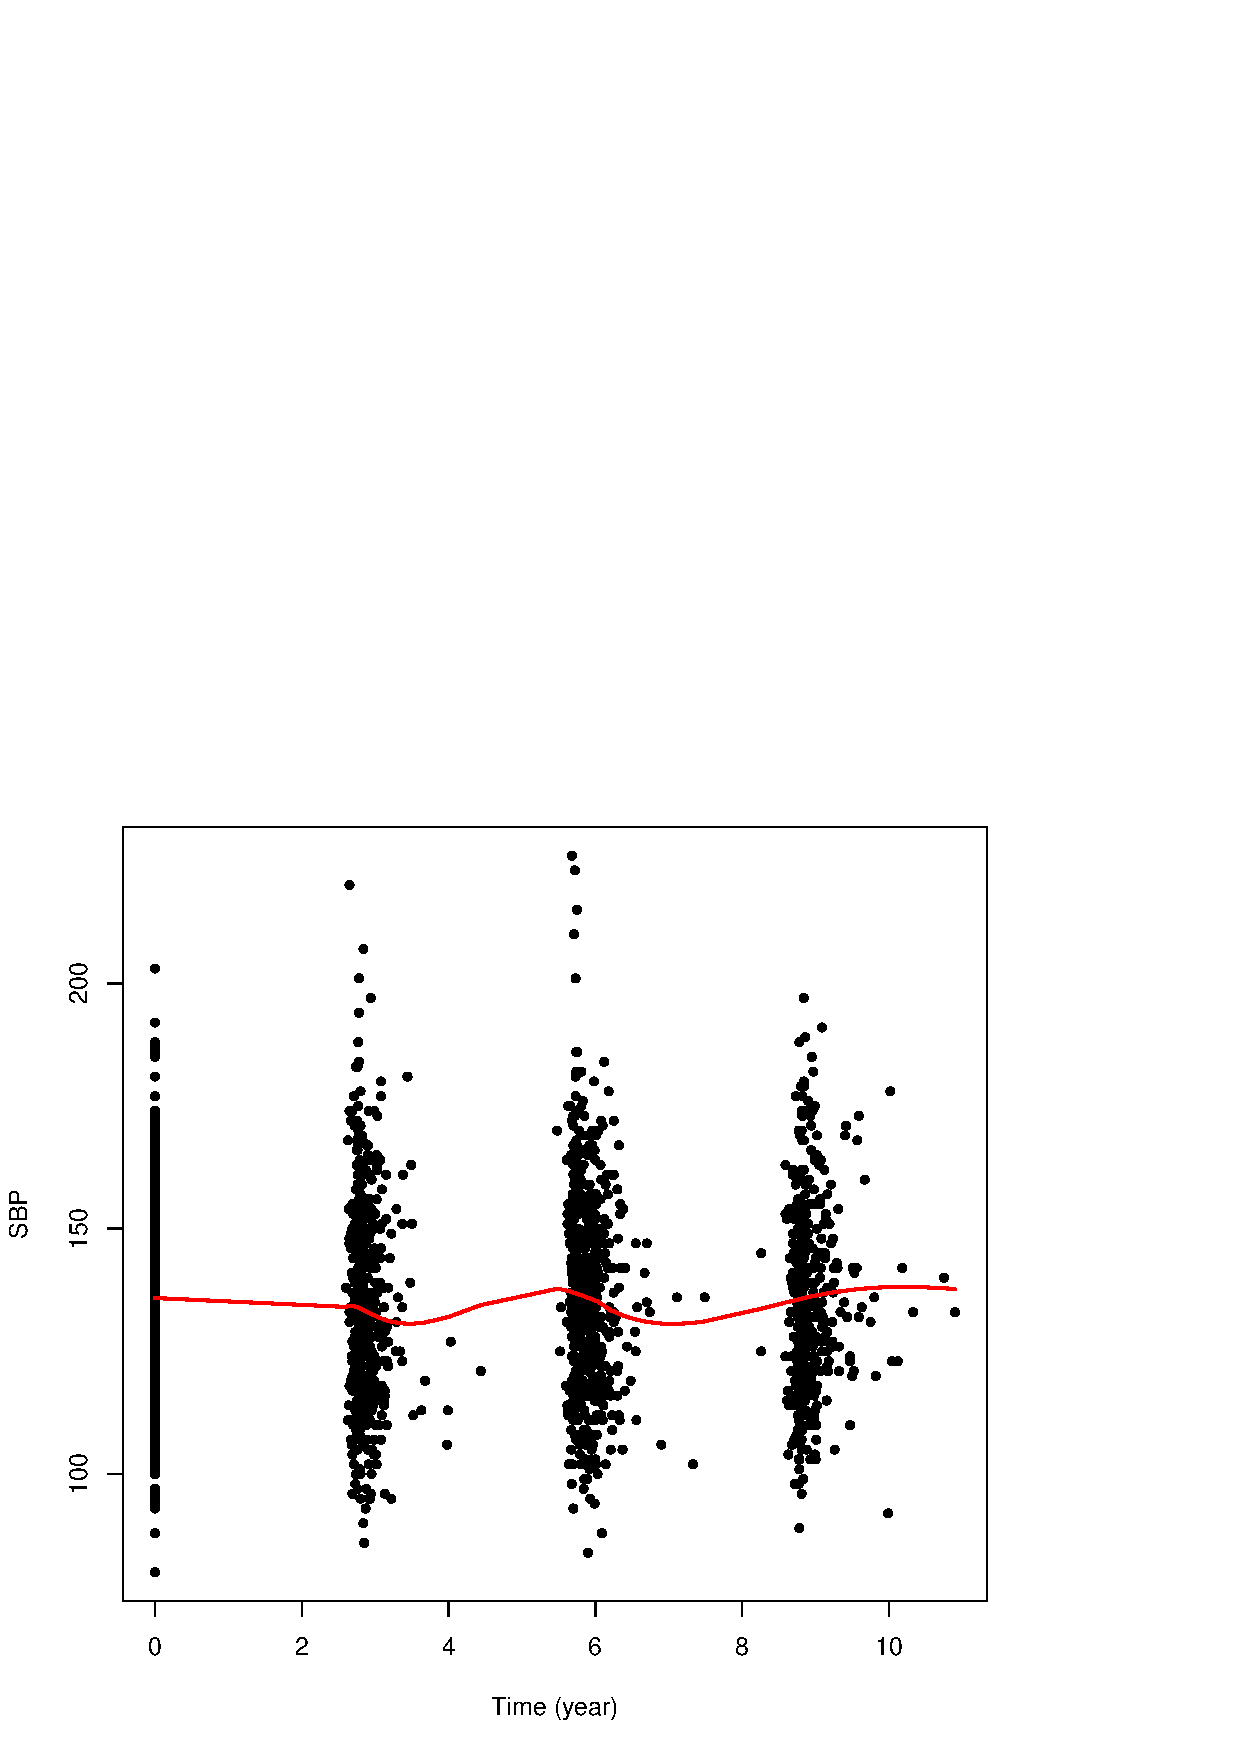
\includegraphics[scale=0.6]{SBP_loess.pdf}
\caption{Scatter plot with LOESS curve of longitudinal SBP measures in the study cohort.}
\label{fig:p2_sbp_loess}
\end{figure}

In data analysis, follow-up time is converted from days to years and the first examination date is set to time 0; baseline age is centered by subtracting the overall mean, and total-cholesterol is standardized to have mean 0 and standard deviation 1. We consider the following QRJM:
\small{
\begin{equation*}\label{eqn:p2data_joint}
\left\{
\begin{array}{l}
sbp_{i}(t) = m_{i}(t) + \varepsilon_{i}(t) = \beta_0 + \beta_1 age_{0i} + \beta_2 chol_i + \beta_3 I_{hyper-med_i}+ \beta_4 t + {u}_{i1} + u_{i2} t + \varepsilon_{i}(t)\\
r_i(t|\mathcal{M}_{it};  \boldsymbol{\gamma}, \alpha) = \sum_{k=1}^3v_i\lambda_kI_k(t)\exp(\gamma_1 I_{male_i} + \gamma_3 I_{smoke_i} + \gamma_4I_{diabetes_i} + \alpha m_i(t))
\end{array}
\right.
\end{equation*}
}
where we assume  $\varepsilon_{i}(t)\sim ALD(0, \sigma, \tau)$. $age_0$ is the baseline age at the first examination, $chol$ stands for the total-cholesterol level (mg/dL), $I_{hyper-med}$ is the variable indicating whether an individual had taken hypertension lowering medication, $t$ is the follow-up time, and $u_{i1}$ and $u_{i2}$ are subject-specific random intercept and slope to account for the within subject correlation and between subject variation. In the recurrent event submodel, we specify a piecewise constant baseline intensity function with three time intervals, where $\lambda_k$ is the hazard rate for time interval $[t_{k-1}, t_{k})$, that is $I_k(t)=1$ if $t\in[t_{k-1}, t_{k})$ and 0 otherwise. Knots $t_1$ and $t_2$, used to define piecewise constant time intervals, are selected as the 33.3\% and 66.7\% percentiles of the ordered follow-up time; while $t_0$ = 0 and $t_3$ is the maximum of follow-up time. We also include a frailty term $v_i$ in the recurrent event model that introduces correlation of multiple CHD events within the same individual. Other model covariates include indicator variables for male ($I_{male}$), ever smoke ($I_{smoke}$), and diabetes mellitus ($I_{diabetes}$). In the QRJM, the true underlying longitudinal measure of SBP is treated as a time dependent covariate in the recurrent event process and $\alpha$ is the association parameter governing the dependence between these two processes. Two chains with diverse initial values are initiated in the Bayesian inference algorithm and the chains are considered to converge if the potential scale reduction factors (PSRF) for all parameters are below 1.1.


\subsection{Inference Results for ARIC data}\label{sec:p2data_results}
Inference results from five different quantiles (0.05, 0.25, 0.50, 0.75, and 0.95) of SBP are shown in Table~\ref{p2realdata_inference} as well as visualized in Figure~\ref{p2_jm_infer}. In the longitudinal SBP process, older participants generally have higher SBP level and the effect of baseline age is consistently positive across all five selected quantiles of SBP. For example, one year increase in baseline age is associated with 0.037 (95\% CI: (0.028, 0.047)) unit increase in the median (i.e., $\tau=0.50$) of standardized SBP in the study cohort when controlling for other covariates. Total cholesterol level is negatively associated with SBP; however, the effects are not significant across all five quantiles. In general, people who took hypertension medications have significantly lower SBP and the effect of taking hypertension medications is larger at higher levels of SBP. Moreover, it is interesting to see that follow-up time has a significantly positive effect on higher quantiles of SBP (i.e., $\tau=0.75$ and 0.95) while for lower quantiles ($\tau=0.05$, 0.25, and 0.50) the effect is not significant. This finding can be an important indication that among the hypertension patients who originally have excessively higher SBP deteriorate even faster than those with lower SBP.

In the recurrent CHD event process, we see all positive association between the five conditional quantiles of SBP and the risk of CHD event, which coincide with our expectation as well as previous findings from ARIC data. However, the degree of association between these two processes varies among the conditional quantiles and is found to be strongest at the conditional median of SBP (relative risk:1.25, 95\% CI: (1.02, 1.53)) among the five selected quantiles. For other regression covariates, diabetic patients are at significantly higher risk of having recurrent CHD event compared with non-diabetic. For example, when controlling for other factors, the risk of having additional CHD event is 2.3 times higher ($\exp(0.85)$, 95\% CI: (1.46, 3.85)) for people with diabetes than those who are free of the disease at $\tau=0.5$. We also observed the posterior effect of diabetes decreases as quantile increases. This indicates that the effect of diabetes on the risk of recurrent CHD event is less important for patients with higher SPB. Although  male patients and ever smokers are also at higher risk of experiencing CHD events, the relative risks are statistically insignificant compared with female and never smokers respectively.

\newpage
\thispagestyle{lscape}
\pagestyle{lscape}
\begin{landscape}
\doublespacing
\begin{table}[H]
\centering
\caption{ARIC data analysis: Parameter estimation and 95\% credible interval (in parenthesis) from QRJM at five quantiles.}
\label{p2realdata_inference}
\resizebox{\linewidth}{!}{
\begin{tabular}{lccccc}
  \hline
  & $\tau=0.05$ & $\tau=0.25$ & $\tau=0.50$ & $\tau=0.75$ & $\tau=0.95$\\
\hline
\multicolumn{6}{c}{\textit{longitudinal SBP process}}  \\
  intercept & -0.374 (-0.478, -0.274) & -0.023 (-0.118, 0.074) & 0.447 (0.352, 0.554) & 0.872 (0.775, 0.978) &1.187 (1.079, 1.300)\\
  age$_0$ & 0.035 (0.026, 0.044) & 0.034 (0.025, 0.044) & 0.037 (0.028, 0.047) & 0.040 (0.030, 0.050) & 0.043 (0.031, 0.052)\\
  total-chol.(mg/dL) & -0.020 (-0.073, 0.033) & -0.026 (-0.081, 0.032) & -0.022 (-0.078, 0.037) & -0.013 (-0.073, 0.047) & -0.022 (-0.076, 0.032)\\
  hypertension medicine & -0.583 (-0.710, -0.467) & -0.652 (-0.773, -0.538) & -0.725 (-0.842, -0.609) & -0.730 (-0.868, -0.593) & -0.787 (-0.924, -0.660)\\
  follow-up time (yr) & 0.008 (-0.003, 0.018) & 0.006 (-0.006, 0.019) & 0.011 (-0.001, 0.022) & 0.016 (0.004, 0.029) & 0.019 (0.005, 0.033)\\
  \multicolumn{6}{c}{\textit{recurrent CHD event process}}  \\
  association & 0.163 (-0.003, 0.332) & 0.207 (0.011, 0.405) & 0.226 (0.019, 0.428) &  0.205 (0.034, 0.374) &0.162 (0.028, 0.288)\\
  male & 0.191 (-0.152, 0.548) & 0.185 (-0.170, 0.528) &  0.160 (-0.187, 0.507) & 0.132 (-0.205, 0.477) & 0.110 (-0.234, 0.458)\\
  ever  smoke & 0.291 (-0.044, 0.641) & 0.271 (-0.070, 0.613) & 0.216 (-0.121, 0.552) & 0.165 (-0.177, 0.493) & 0.163 (-0.184, 0.485)\\
  diabetes & 0.918 (0.424, 1.399) & 0.895 (0.409, 1.376) & 0.850 (0.381, 1.349) & 0.811 (0.352, 1.318) & 0.818 (0.333, 1.301)\\
  $\lambda_1$ & 0.011 (0.010, 0.013) & 0.011 (0.010, 0.013) & 0.011 (0.010, 0.012) & 0.011 (0.010, 0.012) & 0.011 (0.010, 0.012)\\
  $\lambda_2$ & 0.028 (0.020, 0.036) & 0.027 (0.019, 0.035) & 0.026 (0.018, 0.034) & 0.024 (0.017, 0.032) & 0.024 (0.017, 0.032)\\
  $\lambda_3$ & 0.073 (0.037, 0.113) & 0.072 (0.036, 0.111) & 0.067 (0.034, 0.105) & 0.065 (0.033, 0.103) & 0.066 (0.034, 0.103)\\
   \hline
\end{tabular}
}
\end{table}
\end{landscape}

\restoregeometry
\pagestyle{plain}

\newpage
\begin{figure}[H]
\centering
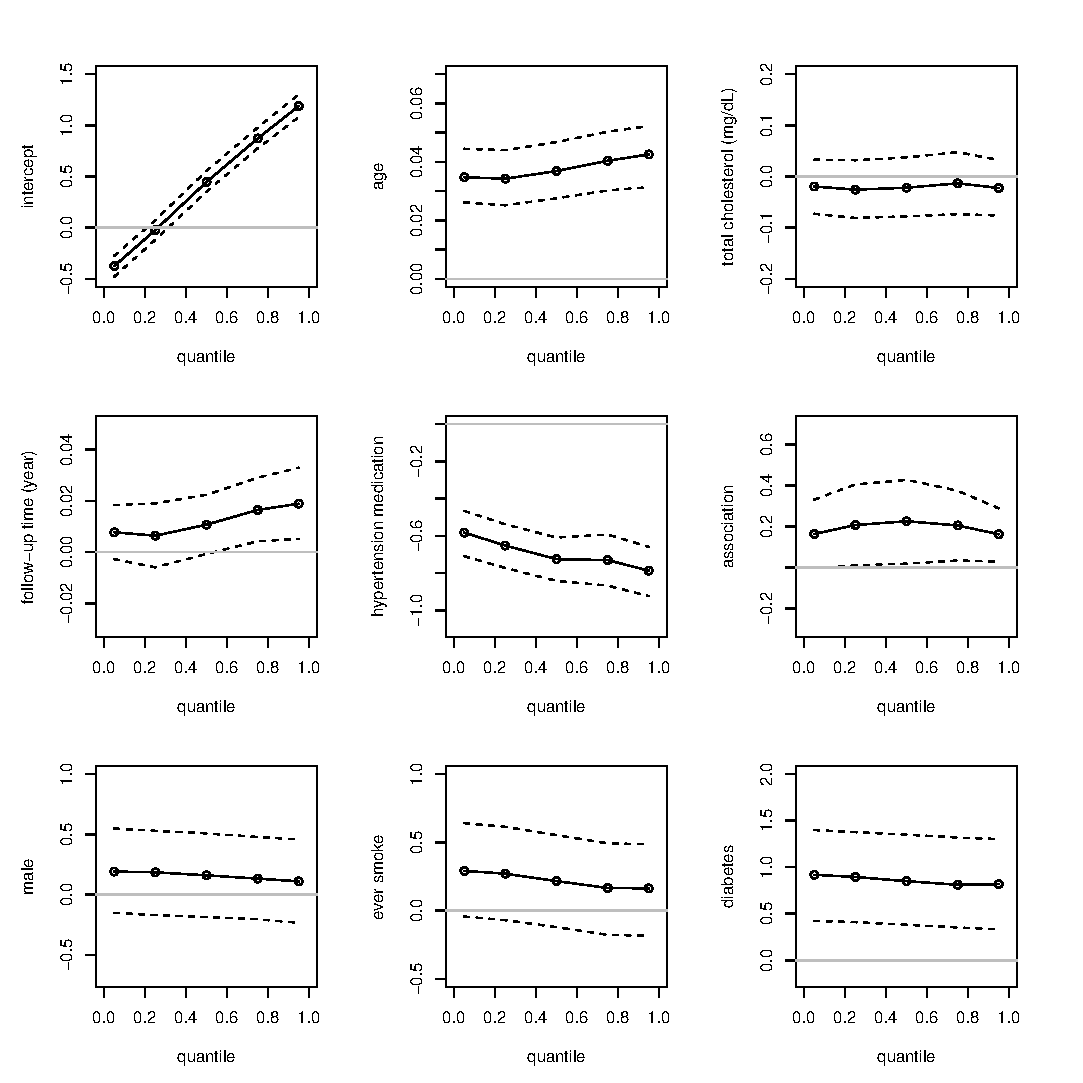
\includegraphics[width=\textwidth]{0.plots/p2_JM_inference_covs.eps}
\caption{ARIC data analysis: Posterior mean (solid line) and point-wise 95\% credible interval (dashed lines) of parameter estimation against different quantiles.}
\label{p2_jm_infer}
\end{figure}



\section{Discussion}\label{sec:p2discussion}
In the application of conventional JM methodologies for longitudinal and recurrent event data, we usually encountered two limitations: first, the normality assumption of the random error in the LMM was not realistic, and no obvious transformation of the longitudinal outcome to produce residual normality was applicable. This limitation is confirmed by our simulation study where LMJM tends to provide biased point estimates as well as lower coverage probabilities for model parameters when the longitudinal data are non-normal. Second, LMJM models only the conditional mean of the outcome; however, in our (and other) clinical research applications, it is more desirable to consider the tails of the biomarker distribution. For example, in our application of the ARIC data, higher level of SBP imposes higher risk of recurrent CHD event and the association between the two outcomes varies according to different conditional quantiles.

Our work on QRJM that uses an LQMM for the longitudinal process provides an alternative and more flexible way for modeling the joint distribution of longitudinal and recurrent event outcomes. The quantile-based estimators are more robust against skewness in the data, and as a result, our approach provides the flexibility to use median or quantile regression instead of mean regression when outliers are concerned. Moreover, QRJM provides a set of estimates at different quantiles of the longitudinal outcome variable, which can have practical meaning when the lower or higher quantile of the outcome is more relevant to health-related questions. In general, we show via simulation and application that QRJM not only inherits the good properties of a LMJM, but adds flexibility to the modeling procedure.

In this work, we developed a Gibbs sampling algorithm to fit the proposed model, where the likelihood function of the longitudinal quantile regression is written under the location-scale representation of the ALD distribution. The proposed algorithm is straightforward to implement in existing Bayesian software. The current version of Gibbs sampler, which is implemented in \textsf{JAGS} software, uses a piecewise constant baseline hazard function in the recurrent event submodel. However, other functional forms can also be considered and the integration of the hazard function can be approximated using Simpson's rule. In the real data application, we illustrate the flexibility of QRJM and its advantages over the LMJM by jointly modeling the risk of developing recurrent CHD event and repeated SBP measurements. QRJM is able to provide us with more informative insights into the disease progression and the association between the two disease processes in terms of various quantile-based estimations.

Our novel extension of JM in using LQMM for the longitudinal outcome finds practical importance in many clinical applications. Studying covariate effects on the conditional mean of the outcome gives us an idea about how treatment and other factors may affect disease progression in the population on average; however, it is limited to be too general and those effects could be dramatically different depending different quantiles of the outcome under investigation. Particularity, higher or lower tail of the longitudinal biomarker is often associated with worse medical condition in patients and leads to higher risk of disease. If treatment effect on tails of the outcome is significantly different from the average effect, treating different groups of patients using the exact same way won't be as effective as we tailor the treatment strategy according to patient-specific situation.

Currently, in the proposed QRJM we only consider an LQMM and a PHM for the longitudinal and recurrent event outcomes respectively. However, other modeling strategies can also be considered to extend the proposed method. For example, for the longitudinal outcome, nonlinear QR \citep{koenker1996interior} or even nonparametric QR \citep{le2005nonparametric} models can be used in stead of linear QR. In the recurrent event submodel, accelerated failure time model can be consider as another parametric formulation for event times and counting process approach is another nonparametric option.



\section*{Appendices}
\addcontentsline{toc}{section}{Appendices}
\renewcommand{\thesubsection}{\Alph{subsection}}
\subsection{Additional simulation results}\label{sec:p2appendix_simulation}
In Scenario 2, data are generated from Laplace distribution (i.e., ALD with $\tau=0.5$). LMJM methods still produce noticeably larger bias and lower CP compared to the true model.

\begin{table}[H]
\centering
\caption{Simulation study: Inference results for data generated from ALD with $\tau$ = 0.50 (Scenario 2).}
\label{tab:p2simsce2}
\begin{tabular}{clccccccc}
\hline
& & \multicolumn{3}{c}{QRJM ($\tau=0.5$)} & & \multicolumn{3}{c}{LRJM}\\
\hline
 & & bias & MSE & CP && bias & MSE & CP \\
 \cline{3-5}  \cline{7-9}
  \multirow{7}{*}{n=250} & $\beta_1$ & 0.005 & 0.007 & 0.97 && 0.006 & 0.008 & 0.97 \\
  & $\beta_2$ & -0.027 & 0.017 & 0.94 && -0.027 & 0.019 & 0.93 \\
  & $\beta_3$ & 0.022 & 0.004 & 0.94 && 0.026 & 0.005 & 0.94 \\
  & $\sigma$ & -0.002 & 0.001 & 0.94 &&  - & - & - \\
  & $\alpha$ & 0.016 & 0.004 & 0.94 && 0.003 & 0.006 & 0.95 \\
  & $\gamma$ & 0.006 & 0.005 & 0.96 && 0.005 & 0.006 & 0.93 \\
  & $r_0$ & 0.011 & 0.013 & 0.95 && 0.011 & 0.014 & 0.95 \\
   \hline
 \multirow{7}{*}{n=500} & $\beta_1$ & -0.001 & 0.004 & 0.93 && -0.001 & 0.005 & 0.93 \\
  & $\beta_2$ & -0.006 & 0.007 & 0.96 && -0.006 & 0.008 & 0.96 \\
  & $\beta_3$ & 0.014 & 0.002 & 0.95 && 0.016 & 0.002 & 0.95 \\
  & $\sigma$ & 0.002 & 0.001 & 0.94 &&  - & - & - \\
  & $\alpha$ & 0.003 & 0.002 & 0.92 && 0.017 & 0.003 & 0.95 \\
  & $\gamma$ & 0.008 & 0.003 & 0.93 && 0.008 & 0.004 & 0.92 \\
  & $r_0$ & -0.019 & 0.008 & 0.93 && -0.022 & 0.008 & 0.95 \\
   \hline
\end{tabular}
\end{table}



In Scenario 3, data are simulated from QRJM with $\tau=0.75$. Results are similar to what we observed when $\tau=0.25$ in Scenario One.

\begin{table}[H]
\centering
\caption{Simulation study: Inference results for data generated from ALD with $\tau$ = 0.75 (Scenario 3).}
\label{tab:p2simsce3}
\adjustbox{max width=\textwidth}{
\begin{tabular}{clccccccccccc}
\hline
& & \multicolumn{3}{c}{QRJM ($\tau=0.75$)} & & \multicolumn{3}{c}{QRJM ($\tau=0.5$)} & & \multicolumn{3}{c}{LRJM}\\
\hline
 & & bias & MSE & CP && bias & MSE & CP & & bias & MSE & CP\\
 \cline{3-5}  \cline{7-9} \cline{11-13}
   \multirow{7}{*}{n=250} & $\beta_1$ & 0.004 & 0.007 & 0.96 && 0.003 & 0.017 & 0.91 && 0.173 & 0.053 & 0.79\\
  &   $\beta_2$ & -0.026 & 0.018 & 0.93 && -1.119 & 1.282 & 0.00 && -1.813 & 3.343 & 0.00\\
  &   $\beta_3$ & 0.025 & 0.004 & 0.93 && -0.119 & 0.022 & 0.65 && 0.001 & 0.012 & 0.92\\
  &   $\sigma$ & -0.003 & 0.001 & 0.93 && -0.333 & 0.111 & 0.00 && - & - & - \\
  &   $\alpha$ & 0.016 & 0.004 & 0.96 && -0.037 & 0.014 & 0.84 && -0.227 & 0.058 & 0.25\\
  &   $\gamma$ & 0.009 & 0.005 & 0.95 && -0.047 & 0.008 & 0.93 && -0.068 & 0.012 & 0.87\\
  &   $r_0$ & 0.010 & 0.013 & 0.96 && 2.155 & 4.781 & 0.00 && 4.469 & 20.237 & 0.00\\
   \hline
  \multirow{7}{*}{n=500} & $\beta_1$ & -0.006 & 0.004 & 0.93 && -0.008 & 0.009 & 0.92 && 0.149 & 0.044 & 0.67\\
  & $\beta_2$ & -0.014 & 0.009 & 0.93 && -1.080 & 1.181 & 0.00 && -1.777 & 3.187 & 0.00\\
  & $\beta_3$ & 0.024 & 0.002 & 0.90 && -0.126 & 0.019 & 0.41 && -0.022 & 0.011 & 0.93\\
  & $\sigma$ & 0.003 & 0.001 & 0.96 && -0.327 & 0.108 & 0.00 && - & - & - \\
  & $\alpha$ & 0.001 & 0.003 & 0.94 && -0.023 & 0.006 & 0.87 && -0.153 & 0.430 & 0.08\\
  & $\gamma$ & 0.004 & 0.003 & 0.94 && -0.041 & 0.005 & 0.87 && -0.069 & 0.010 & 0.77\\
  & $r_0$ & -0.011 & 0.008 & 0.96 && 2.053 & 4.301 & 0.00 && 4.359 & 19.350 & 0.01\\
   \hline
\end{tabular}
}
\end{table}



\newpage
\thispagestyle{lscape}
\pagestyle{lscape}
\begin{landscape}
\doublespacing
\subsection{Summary table of study cohort characteristics}
\begin{table}[H]
\centering
\caption{Baseline characteristics of study cohort with stratification by SBP level}
\label{tab:p2cht_baseline}
\resizebox{\linewidth}{!}{
\begin{tabular}{llcccc}
\hline
& & \multicolumn{3}{c}{SBP groups (mm Hg)} \\
\cline{3-5}
 Characteristics\textsuperscript{$\dagger$} & Total (657) & $<$ 120 (133, 20.2\%)  & [120, 140) (217, 33.0\%)& $\ge$ 140 (307, 46.7\%) & $p$-value\textsuperscript{*}\\
 \hline
 Age & 56.4 (5.8) & 55.0 (5.7) & 55.7 (6.0) & 57.4 (5.4) & $<$0.001\\
 SBP & 135.9 (18.5) & 110.5 (6.9) & 129.2 (5.7) & 151.6 (11.2) & $<$0.001\\
 Cholesterol (mg/dL)& 215.9 (41.7) & 215.1 (42.1) & 214.0 (42.0) & 217.6 (41.7) & 0.60 \\
 Gender (male) & 341 (51.9) & 64 (48.1) & 117 (53.9) & 160 (52.1) & 0.57\\
 Ever smoke (yes) & 379 (57.5) & 81 (60.9) & 126 (58.1) & 172 (56.0) & 0.63\\
 Hypertension medication (yes) & 445 (67.7) & 132 (99.2) & 196 (90.3) & 117 (38.1) & $<$0.001\\
 Diabetes (yes) & 90 (13.7) & 15 (11.3) & 27 (12.4) & 48 (15.6) & 0.38\\
   \hline
   \multicolumn{6}{l}{\textsuperscript{$\dagger$}\footnotesize{mean (sd) for continuous variables and frequency (percentage) for categorical variables.}}\\
   \multicolumn{6}{l}{\textsuperscript{*}\footnotesize{Comparing three SBP groups; ANOVA test for continuous variables and $\chi^2$ test for categorical variables.}}\\
\end{tabular}
}
\end{table}
\end{landscape}

\restoregeometry
\pagestyle{plain}



\newpage
\subsection{\textsf{JAGS} model file}
\textsf{JAGS} model file to fit QRJM of longitudinal and recurrent event data.
{\small
\begin{verbatim}
model{
      k1 <- (1-2*qt)/(qt*(1-qt))
      k2 <- 2/(qt*(1-qt))

      # prior of random effects
      for (i in 1:I){ # I: unique subject id
        # prior for random effects
          u[i] ~ dnorm(0, tau)
      } # end of loop i

      # longitudinal process, BQR mixed model using ALD representation
      for (j in 1:N_l){ # N_l: number of longitudinal observations
          er[j] ~ dexp(sigma)
          mu[j] <- beta1*X1_l[j] + beta2[X2_l[j]] + beta3*t[j] + u[id_l[j]]
          			+ k1*er[j]
          prec[j] <- sigma/(k2*er[j])
          y[j] ~ dnorm(mu[j], prec[j])
      } #end of j loop

    # recurrent events part, baseline hazard is set to constant c
      for(k in 1:I){
        for (l in (s[k]+1):s[k+1]){
          m1[l] <- beta1*X1[k]+beta2[X2[k]]+beta3*Ri1[l]+u[id_r[l]]
          m2[l] <- beta1*X1[k]+beta2[X2[k]]+beta3*Ri2[l]+u[id_r[l]]
          res[l] <- (exp(gamma*W[k]+alpha*m2[l])
                       -exp(gamma*W[k]+alpha*m1[l]))/(alpha*beta3)
          S[l] <- exp(-c*res[l])
          risk[l] <- c*exp(gamma*W[k] + alpha*m2[l])
          L[l] <- pow(risk[l], event[l])*S[l]/1E+08
          zeros[l] ~ dpois(-log(L[l]))
        } # end of l loop
      }#end of k loop

    # priors for other parameters
      alpha ~ dnorm(0, 0.0001)
      beta1 ~ dnorm(0, 0.0001)
      beta2[1] <- 0
      beta2[2] ~ dnorm(0, 0.0001)
      beta3 ~ dnorm(0, 0.0001)
      gamma ~ dnorm(0, 0.0001)
      sigma ~ dgamma(0.001, 0.001)
      c ~ dunif(0.01, 10)
      tau <- pow(var, -2)
      var ~ dunif(0, 1000)
  }
\end{verbatim}
}


%%%%%%%%%%%%%%%%%%%% reference %%%%%%%%%%%%%%%%%%%%
\bibliographystyle{apa}
\addcontentsline{toc}{section}{References}
\bibliography{paper2}

\end{document}